%
% homologie.tex
%
% (c) 2017 Prof Dr Andreas Müller, Hochschule Rapperswil
%
\chapter{Homologie%
\label{chapter:homologie}}
\lhead{Homologie}
\rhead{}
In der elementaren linearen Algebra wird im Zusammenhang mit den
Kirchhoff-Gleichungen gezeigt, wie man zu jedem Graphen eine
minimale Menge linear unabhängiger Zyklen finden kann.
In den Anwendungen wird dies dafür gebraucht, eine linear unabhängige
Menge von Maschen für die Gleichungen von Kirchhoff zu bestimmen.
Es zeigt sich jedoch auch, dass der Begriff des Zyklus sehr viel
allgemeiner formuliert werden kann, und dass sich damit ein algebraisches
Objekt konstruieren lässt, mit welchem sich topologische Eigenschaften
eines Körpers beschreiben lassen.
Der Begriff der Homologie-Gruppen verallgemeinert eine grundlegende
Beobachtung, die schon Euler über Polyeder gemacht hat.

Das Konzept ist aber noch weit tragfähiger.
Im ersten Abschnitt soll gezeigt werden, wie die Idee von Rand-Operatoren,
die für die Definition der Homologie-Vektorräume grundlegen sind, 
auch in ganz anderen Bereichen der Mathematik auftreten.

%
% beispiele.tex
%
% (c) 2020 Prof Dr Andreas Müller, Hochschule Rapperswil
%
\subsection{Beispiele
\label{subsection:qam:beispiele}}
Die Quadratur-Amplituden-Modulation ermöglicht, im Vergleich zur
Trägerfrequenz langsam veränderliche zweidimensionale Signale zu
übertragen und wieder zu rekonstruieren.
Der besondere Nutzen dieser Technik ist jedoch, dass sie viele
ältere Modulationsverfahren als Spezialfälle enthält, wie in
diesem Abschnitt gezeigt werden soll.

\subsubsection{Amplitudenmodulation}
{\em Amplitudenmodulation} konnten wir verstehen, bevor wir $Q(t)$ kannten,
sie ist der Spezialfall $Q(t)=0$.
Für ein Audiosignal $A(t)$ mit $A(t)<1$ wird $I(t)=1+A(t)$ verwendet.
Das in Europa weitgehend bereits durch Digitalradio ersetzte 
Mittelwellenradio (AM) verwendet Amplitudenmodulation.
Bis 2025 werden in Europa alle Radiostationen digitalisiert, damit
wird AM für den Rundfunk aussterben.

\subsubsection{Phasenmodulation}
\begin{figure}
\centering
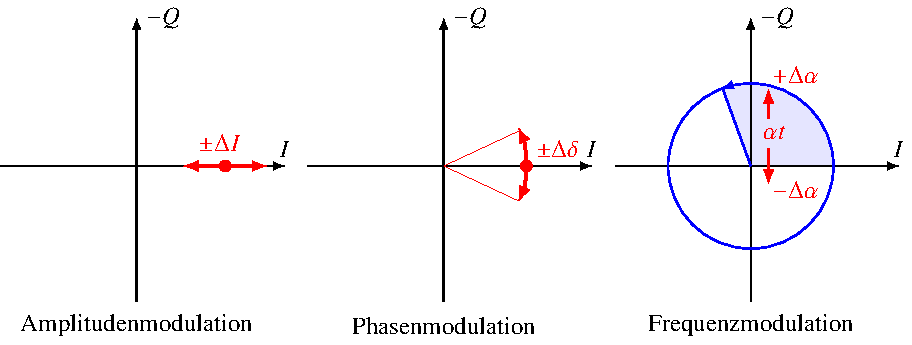
\includegraphics{applications/qam/images/amfmpm.pdf}
\caption{Amplitudenmodulation (links), Phasenmodulation (mitte) und
Frequenzmodulation in der $I$-$Q$-Ebene.
Frequenzmodulation ensteht durch eine Drehung in der $I$-$Q$-Ebene
mit der Kreisfrequenz der gewünschten Frequenzänderung.
\label{qam:figure:amfmpm}}
\end{figure}
Statt der Amplitude kann auch die Phase des Trägersignals moduliert werden.
Dazu muss $\omega t$ ersetzt werden durch $\omega t + \delta$.
Der konstante unmodulierte Vektor $\vec{v}_0$ in der $I$-$Q$-Ebene erzeugt
das modulierte Signal
\begin{align*}
D_{\omega t + \delta}
\vec{v}_0
&=
D_{\omega t}\underbrace{D_{\delta} \vec{v}_0}_{\displaystyle=\vec{v}(t)}.
\end{align*}
Eine Phasenänderung um den Winkel $\delta$ entsteht also dadurch, dass
man den Vektor $\vec{v}_0$ in der $I$-$Q$-Eben um $\delta$ dreht.
Dieses Modulationsverfahren heisst {\em Phasenmodulation}.
Abbildung~\ref{qam:figure:amfmpm} zeigt in der Mitte die Transformation
in der $I$-$Q$-Ebene, die Phasenmodulation bewirkt.

Mit reiner Amplitudenmodulation lässt sich kein Stereosignal übertragen.
Sind $L(t)$ und $R(t)$ die beiden Stereokanäle, dann erfolgt die
Amplitudenmodulation typischerweise mit $I(t)=1+L(t)+R(t)$,
wobei man wieder $L(t)+R(t)<1$ voraussetzen muss.
Ein reiner AM-Empfänger wird also nur das Audio-Signal $A(t)=L(t) + R(t)$
empfangen.

Um die Stereoinformation zu übermitteln, muss zusätzlich die Differenz
$L(t)-R(t)$ übermittelt werden.
Das C-QUAM Verfahren ({\bf C}ompatible {\bf Qu}adrature {\bf A}mplitude
{\bf M}odulation) verwendet dafür $Q(t)=L(t)-R(t)$.
Man darf annehmen, dass $L(t)-R(t)$ klein ist.
Dann befinden sich die Punkte $(I(t),Q(t))$ immer in der
Nähe der $I$-Achse, was sich in einer kleinen Verschiebung
\[
\delta = \arctan\frac{Q(t)}{I(t)} = \arctan\frac{L(t)-R(t)}{1+L(t)+R(t)}
\]
der Phase des übermittelten Signals äussert.
Der Betrag des Vektors $\vec{v}(t)$ ist dagegen
\begin{align*}
|\vec{v}(t)|
&=
\sqrt{
(1+L(t)+R(t))^2
+
(L(t)-R(t))^2
}
=
(1+L(t)+R(t))
\sqrt{
1+
\biggl(
\frac{L(t)-R(t)}{1+L(t)+R(t)}\biggr)^2
}
\\
&\simeq 1+L(t)+R(t),
\end{align*}
weil der zweite Summand unter der Wurzel klein ist.
Die $Q$-Komponente ändert also nicht wirklich etwas am Signal, welches
ein AM-Empfänger empfängt.

Um dem Emfpänger zu signalisieren, dass eine Stereoübertragung
vorliegt, wird $Q(t)$ zusätzlich ein Pilotton von 25\,Hz hinzugefügt.
Da nicht C-QUAM-taugliche Empfänger die Phasenschwankungen nicht erkennen
können, werden sie vom Pilotton auch nicht gestört.

\subsubsection{Frequenzmodulation}
Bei der {\em Frequenzmodulation} des UKW-Radios wird die Trägerfrequenz
im Takt des zu übertragenden Tonsignals verändert.
Lässt sich dies auch mit Hilfe der Signale $I(t)$ und $Q(t)$
beschreiben?
Welche Funktionen $I(t)$ und $Q(t)$ muss man wählen?

Ist das zu übertragende Audiosignal $0$, dann wird nur der unveränderte
Träger ausgestrahlt.
Dies lässt sich dadurch erreichen, dass man für $\vec{v}(t)$ den
konstanten Vektor $\vec{v}(t)=\vec{v}_0=(1,0)^t$ wählt.

Das ausgestrahlte Signal $s(t)$ entsteht als erste Komponente
des Vektors $D_{\omega t}\vec{v}(t)$.
Für konstantes $\vec{v}(t)=\vec{v}_0$ oszilliert es mit der Kreisfrequenz
$\omega$.
Will man, dass es schneller oszilliert, dann muss die Frequenz $\omega$
erhöht werden.
Möchte man die Frequenz um $\alpha$ steigern, dann muss man $\omega$
durch $\omega+\alpha$ ersetzen.
Das modulierte Signal ist dann
\[
\begin{pmatrix}
s(t)\\c(t)
\end{pmatrix}
=
D_{(\omega+\alpha)t} \vec{v}_0
=
D_{\omega t} \underbrace{D_{\alpha t} \vec{v}_0}_{\displaystyle=\vec{v}(t)}.
\]
Dies ist gleichbedeutend damit, dass man den Vektor $\vec{v}_0$ in der
$I$-$Q$-Ebene mit der Winkelgeschwindigkeit $\alpha$ dreht und so
$\vec{v}(t)$ erhält.
Daraus liest man ab, dass für die Signale $I(t)$ und $Q(t)$
\begin{equation}
\begin{pmatrix}I(t)\\Q(t)\end{pmatrix}
=
D_{\alpha t}\vec{v}_0
\qquad\Rightarrow\qquad
\left\{
\quad
\begin{aligned}
I(t)&=\cos\alpha t\\
Q(t)&=\sin\alpha t
\end{aligned}
\right.
\end{equation}
gilt.
Insbesondere kann man auch die Frequenzmodulation mit der
Quadratur-Amplituden-Modulation realisieren.
Abbildung~\ref{qam:figure:amfmpm} zeigt rechts symbolisch die
Kreisbewegung in der $I$-$Q$-Ebene, die Frequenzmodulation bewirkt.

\subsubsection{Analoges Farbfernsehen}
Die Entwicklung des analogen Farbfernsehens sah sich vor die Aufgabe 
gestellt, zusätzlich zur bereits im Schwarz-Weiss-Fernsehen übertragenen
Helligkeit (Luminanz, Y) die Farbinformation zu übermitteln.
Üblich ist dabei die Verwendung des YUV-Farbraumes, für den die zusätzlichen
Signale $U=R-Y$ und $V=B-Y$ benötigt werden, welche die Farbinformation
codieren.
Für ein farbloses Bild sind $U=0$ und $V=0$.

Das Problem ist also, zusätzlich zum Luminanzbild, welches bereits
amplitudenmoduliert übertragen wird, den Farbvektor $(U,V)^t$ zu
übertragen.
Es liegt daher nahe, dafür die Quadratur-Amplituden-Modulation zu
verwenden.
Im in Europa üblichen PAL-System wurde für den Träger für das Farbsignal
die Frequenz 4.43361875\,MHz verwendet.
Da ein Phasenfehler im Empfänger zu einer Drehung des Farbvektors
und damit zu einer auffälligen Verschiebung der Farben auf dem Farbkreis
führen würde, muss der Sender dem Empfänger die genaue Phase mitteilen.
Am Anfang jeder Zeile wird daher eine etwa zehn Perioden langer ``PAL-Burst''
übermittelt, den der Empfänger dazu verwenden kann, die Phase des
Farbträgers zu bestimmen.

Zusätzlich invertiert das PAL-System die Phase des Farbträgers
aufeinanderfolgender Zeilen, so dass sich Farbfehler durch Phasenfehler
auf aufeinanderfolgenden Zeilen wegmitteln.
Im PAL-System steht also Farbinformation jeweils nur für Paare von Zeilen
zur Verfügung und nur mit einer Dichte, die durch die Frequenz des Farbträgers
begrenzt ist.
Die effektive Farbauflösung eines PAL-Farbfernsehbildes ist daher halb so
gross wie die Helligkeitsauflösung.
Da auch die Farbauflösung des menschlichen Auges kleiner ist als die
Helligkeitsauflösung, ist diese Einschränkung des Systems von Auge nicht 
erkennbar.

\subsubsection{FSK und PSK}
Für die digitale Signalübertragung braucht man minimal die Fähigkeit,
zwei Zustände zu übermitteln, die man aber exakt wiedererkennnen können muss.
Frequency-Shift-Keying (FSK) ist ein Verfahren, welches zwei digitale Zustände
durch verschiedene Frequenzen codiert, es ist also ein
Frequenzmodulationsverfahren, von dem im vorangegangenen Abschnitt
bereits gezeigt wurde, wie es mit der Quadratur-Amplituden-Modulation
realisierbar ist.

Phase-Shift-Keying (PSK) verwendet stattdessen eine Phasenverschiebung
des Tragersignals.
Eine Phasenverschiebung um den Winkel $\varphi$ kann realisiert werden,
indem man eine Drehung um den Winkel $\varphi$ vorschaltet, also die
Drehmatrix $D_{\varphi}$ einfügt.
Besonders einfach ist eine Phasenverschiebung um den Winkel
$\varphi=180^\circ$, 
\[
D_{\varphi}
=
\begin{pmatrix}
\cos180^\circ&          - \sin180^\circ \\
\sin180^\circ& \phantom{-}\cos180^\circ
\end{pmatrix}
=
-E.
\]
Diese Phasenverschiebung wird also dadurch realisiert, dass man das
Vorzeichen von $I$ und $Q$ ändert.
Verwendet man den Vektor $(1,0)^t$ zur Codierung einer logischen
$\texttt{0}$, dann codiert der Vektor $(-1,0)^t$ eine logische $\texttt{1}$.
Auch PSK ist also mit Quadratur-Amplituden-Modulation realisierbar.

\subsubsection{Quantisierte QAM}
Mit Quadratur-Amplituden-Modulation lässt sich ein beliebiger Vektor
in der $I$-$Q$-Ebene übertragen.
Bei PSK wurden nur die Punkte $(1,0)$  und $(-1,0)$ in der $I$-$Q$-Ebene
verwendet.
Nach der Demodulation erhält man Vektoren, die wegen Fehlern nicht
exakt mit den ursprünglichen Vektoren übereinstimmen.
Da man aber nur die beiden logischen Zustände unterscheiden können muss,
kann man alle Vektoren mit $I>0$ als logische \texttt{0} decodieren
und Vektoren mit $I<0$ als logische \texttt{1}.

Statt nur zwei Zustände \texttt{0} und \texttt{1} zu codieren, könnte man
ein grössere Zahl von Punkten in der $I$-$Q$-Ebene verwenden, wie in
Abbildung~\ref{figure:qam:konstellation} dargestellt.
Die Punkte werden auch {\em Symbole} genannt.
Ein empfangener Vektor wird wegen Übertragungsfehlern nicht exakt mit
dem ursprünglichen Vektor übereinstimmen.
Zur Decodierung suchen wir dasjenige Symbol, welches dem Vektor am
nächsten liegt.
Man teilt also die Ebene in Teilgebiete $T_{\vec{v}_k}\subset \mathbb R^2$
zu jedem Symbol $\vec{v}_k$ auf.
Fällt der empfangene Vektor $\hat{v}$ in das Teilgebiet des Symbols
$\vec{v}_k$, also $\hat{v}\in T_{\vec{v}_k}$, dann decodieren wir ihn
als das Symbol $\vec{v}_k$.

\begin{figure}
\centering
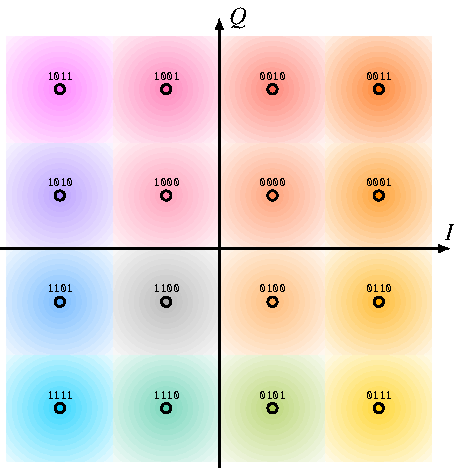
\includegraphics{applications/qam/images/konstellation.pdf}
\caption{Konstellationsdiagramm für quantisierte QAM mit 16 verschiedenen
Symbolen.
Mit jedem Symbol werden vier Bit codiert.
Zu jedem Symbol gehört ein quadratisches Gebiet gleicher Farbe.
Fällt der empfangene Vektor in eines dieser Gebiete, wird er als
das zugehörige Symbol decodiert.
\label{figure:qam:konstellation}}
\end{figure}

Im Beispiel der Abbildung~\ref{figure:qam:konstellation} können 16 
verschiedene Vektoren unterschieden werden, die man mit vierstelligen
Binärzahlen identifizieren kann.
Mit jedem Symbol werden also vier Bit übertragen.
Dieses Verfahren heisst auch 16-QAM und wird bei DVB-T verwendet.

Die Punkte-Menge $\vec{v}_k$ heisst auch die {\em Konstellation}
des Verfahrens.
Durch feinere Aufteilung können mehr Bits pro Symbol übertragen werden,
wie in Tabelle~\ref{table:qam:xqam} zusammengstellt.
Abbildung~\ref{figure:qam:analyzer} zeigt, wie sich die Messung eines 256-QAM 
Signals auf einem Vector Signal Analyzer darstellt.

Für ungerade Potenzen von $2$ kann das Konstellationsdiagramm kein
Quadrat sein.
Für $k$ ungerade kann man aber $2^k$ Punkte erhalten, indem man
dem Quadrat der $2^{k-1}$ Punkte der Konstellation von $2^{k-1}$-QAM
vier Rechtecke mit jeweils $2^{k-1}/4=2^{k-3}$ Punkten hinzugefügt, daraus
ergibt sich eine Konstellation mit
$2^{k-1}+4\cdot 2^{k-3}=2^{k-1}+2^{k-1}=2^k$
Punkten (Abbildung~\ref{qam:figure:qam-konstellation} Mitte).
In diesem hat das Konstellationsdiagramm also die Form
eines Kreuzes mit breite $2^{(k-1)/2}$ und Armlänge
$\frac32\cdot 2^{(k-1)/2}$.
Diese Konstellation wird manchmal auch Cross-QAM genannt.

\begin{table}
\centering
\begin{tabular}{rrcrl}
\hline
Bits&Symbole&Konstellation&Name&Anwendung\\
\hline
   2&      4&$  2\times   2$      &    4-QAM&DVB-S       \\
   4&     16&$  4\times   4$      &   16-QAM&V.29, DVB-T \\
   6&     64&$  8\times   8$      &   64-QAM&DVB-C, DVB-T\\
   8&    256&$ 16\times  16$      &  256-QAM&DVB-C       \\
  10&   1024&$ 32\times  32$      & 1024-QAM&            \\
  12&   4096&$ 64\times  64$      & 4096-QAM&DVB-C2, G.hn\\
  15&  32768&$128\times 256$ Kreuz&32767-QAM&ADSL        \\
\hline
\end{tabular}
\caption{Verschiedene Konstellationen für quantisierte QAM mit Anwendungen.
\label{table:qam:xqam}}
\end{table}

\begin{figure}
\centering
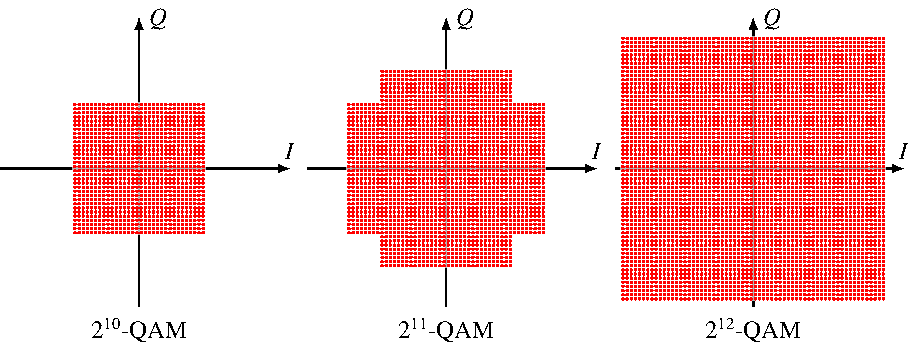
\includegraphics{applications/qam/images/qam.pdf}
\caption{Konstellationsdiagramme für $2^k$-QAM für verschiedene Werte von $k$.
\label{qam:figure:qam-konstellation}}
\end{figure}

\begin{figure}
\centering
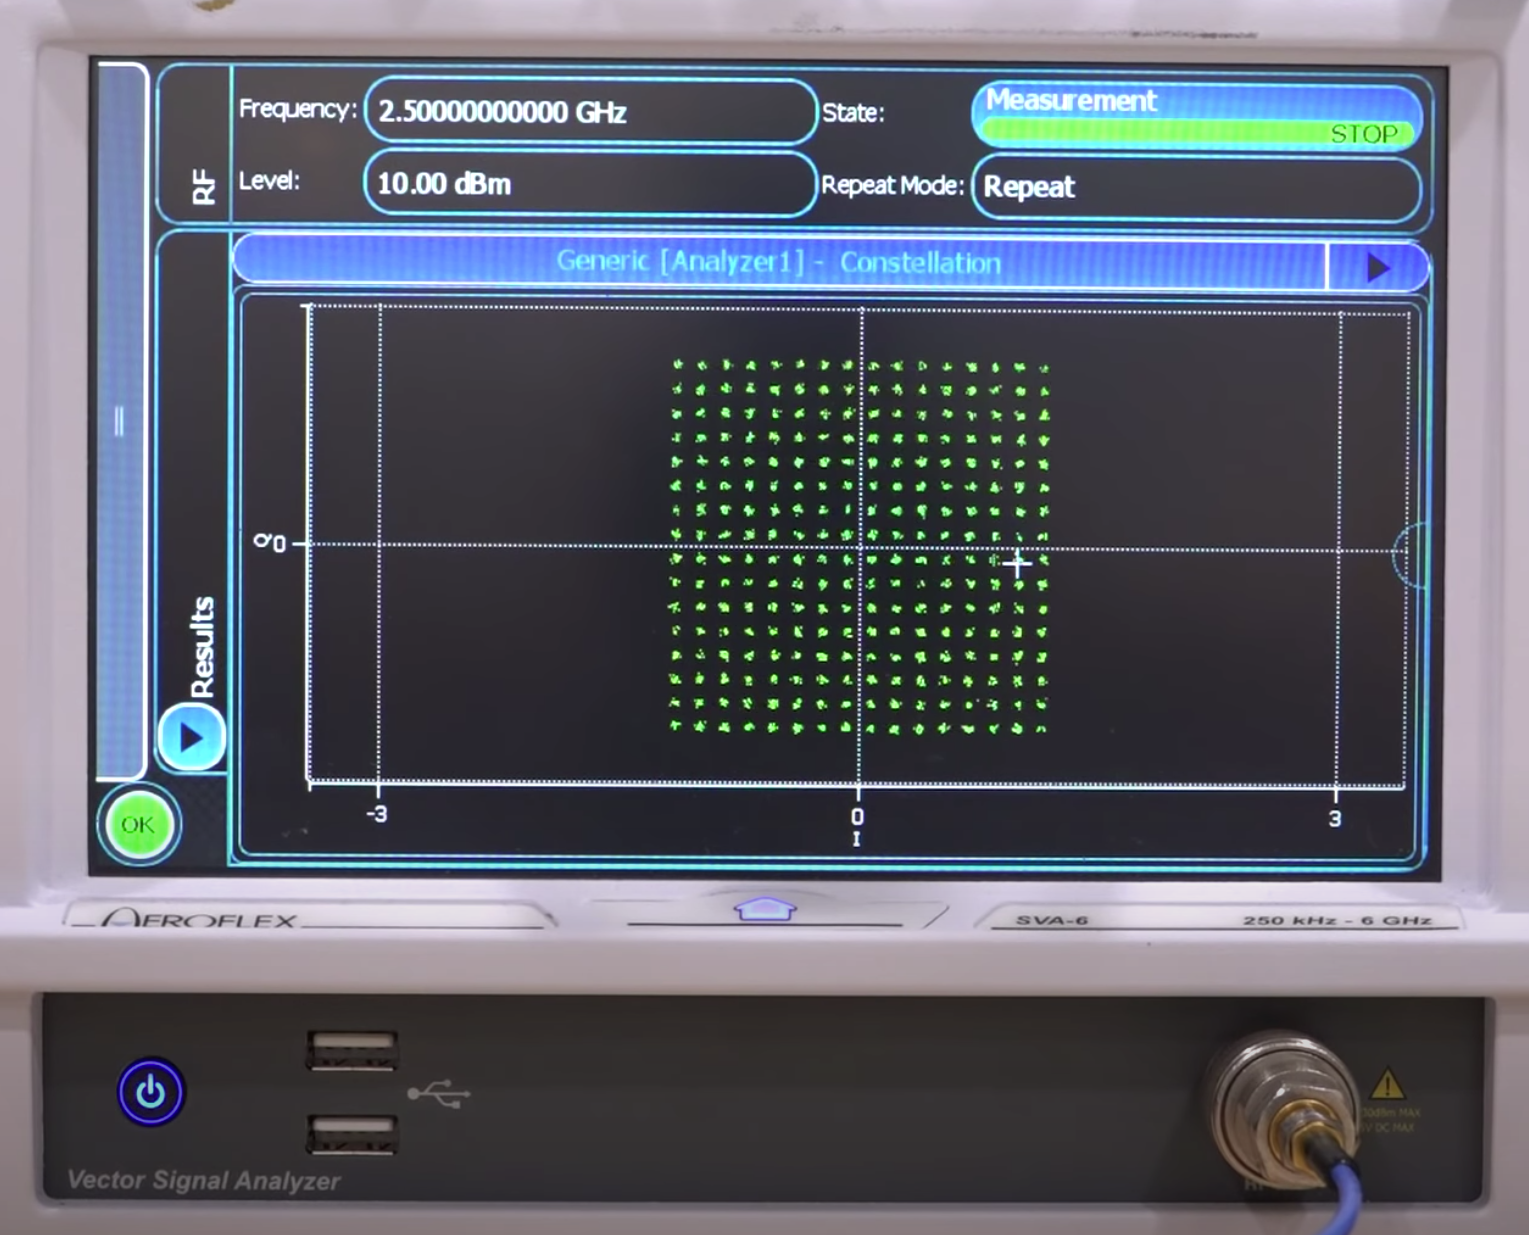
\includegraphics[width=1.0\hsize]{applications/qam/images/analyzer.png}
\caption{Messung des Konstellationsdiagramms eines 256-QAM Signals
mit einem Vector Signal Analyzer.
Man beachte die Beschriftung der Achsen mit \texttt{I} und \texttt{Q}.
(Ausschnitt aus dem Video \url{https://www.youtube.com/watch?v=uV3O3tpjmS8}
bei 26:36).
\label{figure:qam:analyzer}}
\end{figure}

\subsubsection{$n$-PSK}
Analog zum Vorgehen bei der quantisierten QAM kann auch PSK diskretisiert
werden.
Als Konstellationsdiagramm für $n$-PSK dienen $n$ Punkte auf einem Kreis,
die durch einen Winkel $2\pi/n$ getrennt sind.
In Abbildung~\ref{figure:qam:psk} ist das Konstellationsdiagramm für
$8$-PSK dargestellt.
\begin{figure}
\centering
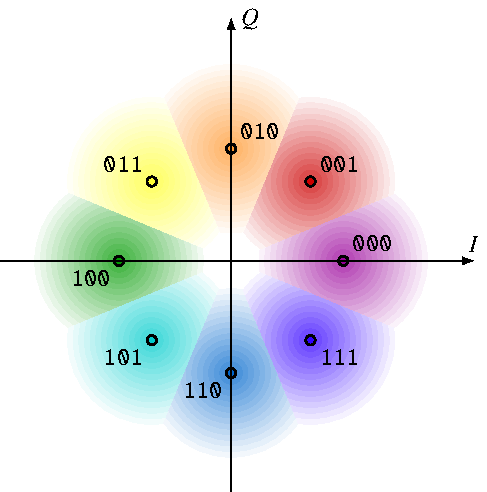
\includegraphics{applications/qam/images/psk.pdf}
\caption{Konstellationsdiagramm für 8-PSK 
\label{figure:qam:psk}}
\end{figure}

\subsubsection{Software Defined Radio}
Die vorangegangenen Beispiele haben illustriert, dass die
Quadratur-Amplituden-Modulation jedes besprochene Modulationsverfahren
realisieren kann.
Es ist nur nötig, einen Sender zu bauen, der Inputs $I(t)$ und $Q(t)$
entgegennimmt, die Modulation mit der Matrix $D_{\omega t}$ vornimmt
und das resultierende Signal $s(t)$ aussendet.
Auf der Empfängerseite braucht man eine physikalische Realisierung
der Matrix $D_{\omega_r t}$ und des Tiefpasses, der die demodulierten
Signal $\hat{I}(t)$ und $\hat{Q}(t)$ ausgibt.
Die Decodierung zum Beispiel als amplitudenmoduliertes Sprachsignal,
als frequenzmoduliertes Musiksignal oder als digitales 16-QAM-Signal
kann danach ausschliesslich in Software erfolgen.
Die Modulationsart eines solchen sogenannten {\em Software Defined Radio (SDR)}
wird also durch die Software definiert, welche die Signale $I(t)$ und $Q(t)$
erzeugt bzw.~die Signale $\hat{I}(t)$ und $\hat{Q}(t)$ analysiert.
SDR ermöglicht dem interessierten Hacker auch exotische Experimente,
wie das in Abbildung~\ref{qam:figure:digital} dargestellte fiktive
digitale Modulationsverfahren.

\begin{figure}
\centering
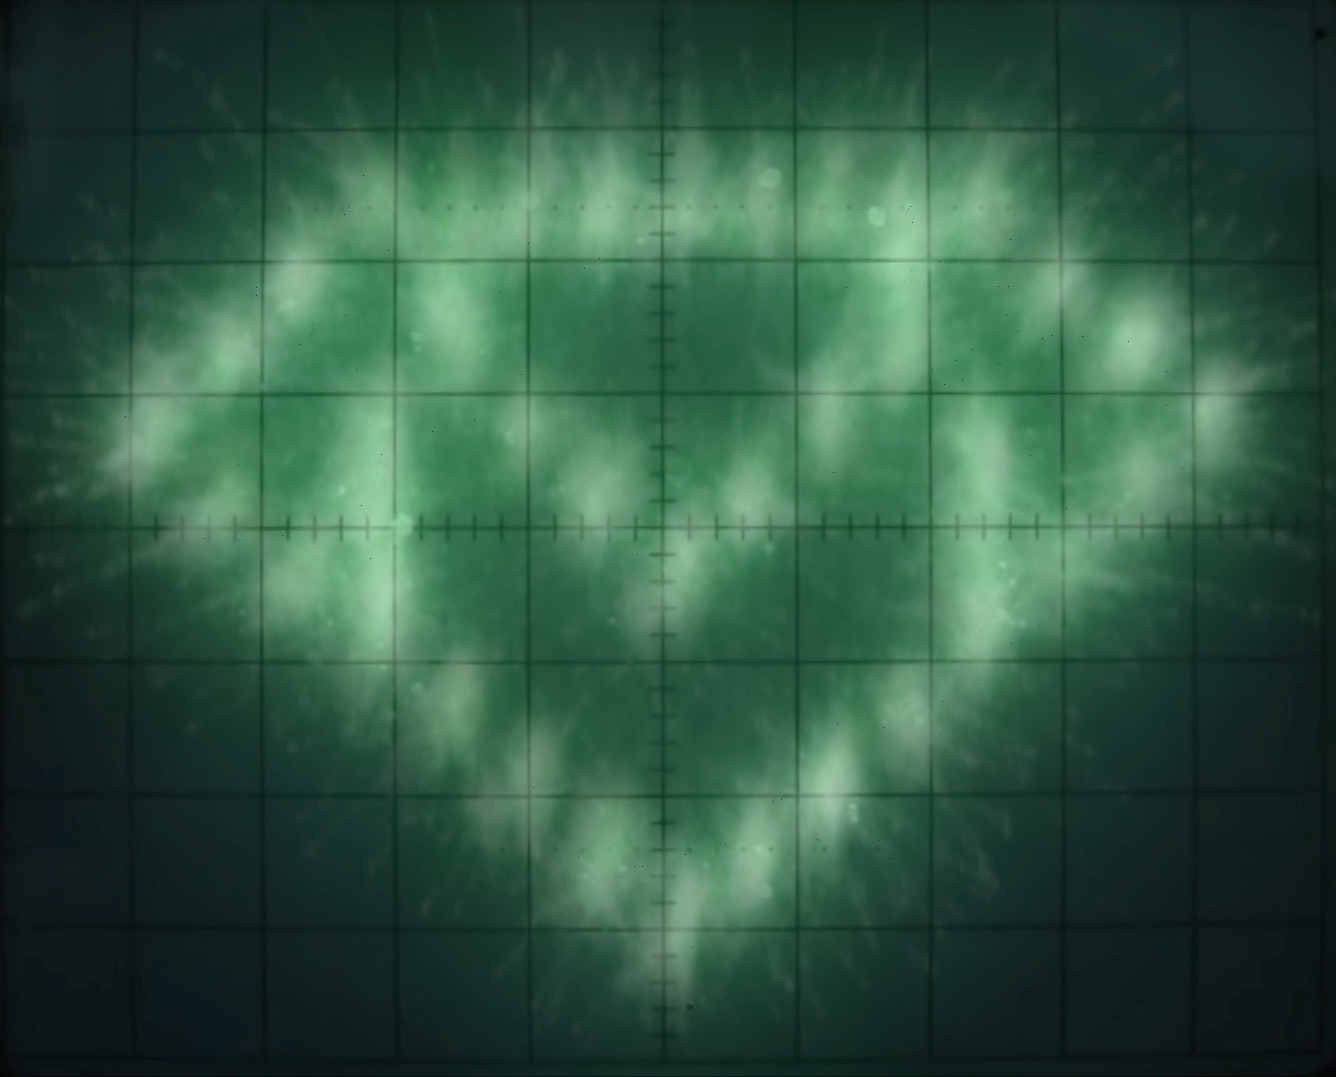
\includegraphics[width=0.7\hsize]{applications/qam/images/digital.jpg}
\caption{Konstellationsdiagramm für ein fiktives digitales
Modulationsverfahren, welches nur Punkte eines MathMan-Logos als
Symbole verwendet.
\label{qam:figure:digital}}
\end{figure}




\section{Kern und Bild}
Seien $U$ und $V$ Vektorräume über $\mathbb R$ und sei $\varphi\colon U\to V$
eine lineare Abbildung.
Dann sind die Mengen
\begin{align*}
\operatorname{ker}\varphi&=\{u\in U\,|\, \varphi(u) = 0\}
\\
\operatorname{im}\varphi&=\{\varphi(u)\,|\, u\in U\}
\end{align*}
Vektorräume.
In der Tat folgt aus $u_1,u_2\in\operatorname{ker}\varphi$
und $\lambda\in\mathbb R$
\begin{align*}
\varphi(u_1+u_2)&=\varphi(u_1)+\varphi(u_2) = 0
&
&\Rightarrow&
u_1+u_2&\in\operatorname{ker}\varphi
\\
\varphi(\lambda u_1)&=\lambda\varphi(u_1)
&
&\Rightarrow&
\lambda u_1&\in\operatorname{ker}\varphi
\end{align*}
was beweist das $\operatorname{ker}\varphi$ ein Vektorraum ist.
Für $\operatorname{im}\varphi$ nehmen wir zunächst
$v_1,v_2\in\operatorname{im}\varphi$.
Dann gibt es Vektoren $u_1,u_2\in U$ derart, dass
$\varphi(u_1)=v_1$ und $\varphi(u_2)=v_2$.
Dann folgt
\begin{align*}
v_1+v_2&=\varphi(u_1)+\varphi(u_2)=\varphi(u_1+u_2)
&
&\Rightarrow&
v_1+v_w&\in\operatorname{im}\varphi
\\
\lambda v_1&=\lambda\varphi(u_1)=\varphi(\lambda u_1)
&
&\Rightarrow&
\lambda v_1&\in\operatorname{im}\varphi,
\end{align*}
was wieder beweist, dass $\operatorname{im}\varphi$ ein Vektor ist.
Es ist klar dass $\operatorname{ker}\varphi\subset U$ und
$\operatorname{im}\varphi\subset V$.

\section{Quotientenraum}
\rhead{Quotientenraum}
Sei jetzt $V$ ein reeller Vekor und $U\subset V$ ein Unterraum.
Dann können wir einen neuen Vektorraum $V/U$ wie folgt definieren.
Die Element von $V/U$ sind Teilmengen der Form
\[
\tilde v = \{v+u\,|\, u\in U\}.
\]
Offenbar ist $\tilde v_1=\tilde v_2$ wenn $v_1-v_2\in U$.
Wir müssen ausserdem die Vektorraum-Operationen definieren.
Es ist naheliegend
\begin{align*}
\tilde v_1+\tilde v_2
&=
\{ v_1+v_2+u\,|\, u\in U\}
\\
\lambda \tilde v_1
&=
\{\lambda v_1+u\,|\, u\in U\}.
\end{align*}
zu setzen, doch wir müssen sicherstellen dass eine andere Wahl
der Repräsentanten $v_i$ auf die gleichen Mengen führt.
Seien also $v_1'$ und $v_2'$ andere Repräsentanten, es gilt also
$v_1'-v_1\in U$ and $v_2'-v_2\in U$.
Dann gilt
\begin{align*}
\{v_1 + v_2 + u\,|\, u\in U\}
&=
\{v_1' + \underbrace{v_1-v_1'}_{\displaystyle\in U}
+ v_2' + \underbrace{v_2-v_2'}_{\displaystyle\in U}
+ u\,|\, u\in U\} = \{v_1'+v_2'+u\,|\, u\in U\}
\\
\{\lambda v_1 + u\,|\, u\in U\}
&=
\{\lambda v_1' + \underbrace{\lambda(v_1-v_1')}_{\displaystyle \in U}+u
\,|\, u\in U\}
=
\{\lambda v_1' + u\,|\, u\in U\}
\end{align*}
Damit ist gezeigt, dass die Vektorraumoperationen in $V/U$ wohldefiniert
sind.

Jetzt muss aber auch noch gezeigt werden, dass die Axiome für einen
Vektorraum erfüllt sind.
Die Rechenregeln wie das Assoziativgesetz oder das Distributivgesetz
folgen jetzt unmittelbar daraus, dass die Rechenoperationen mit Hilfe
von Repräsentationen definiert sind, und für diese gelten die
genannten Gesetze.
Das gilt auch für den Nullvektor, der Repräsentant von $U$ ist.

Die Darstellung von Elementen von $V/U$ mit Hilfe von Repräsentanten
bedeutet auch, dass es eine Abbildung $V\to U$ gibt, die definiert
ist durch
\[
\pi \colon V\to U: v\mapsto \tilde v=\{v+u\,|\, u\in U\}\in V/U.
\]
Auch hier folgt aus den Eigenschaften des Rechnens mit Repräsentaten,
dass $\pi$ eine lineare Abbildung von Vektorräumen ist.
Ausserdem ist das Bild von $\pi$ die ganzge Menge,
$\operatorname{im}\pi = V/U$.

\begin{definition}
Der Vektorraum $V/U$ heisst der Quotient von $V$ nach dem Unterraum $U$,
$\pi$ heisst die (kanonische) Projektion.
\end{definition}

Geometrisch kann man sich den Quotientenraum so vorstellen:
Die Mengen $v+U$ mit $v\in V$ sind parallel verschobene Kopien des
Unterraumes $U$.
Im Quotienten werden alle $v$ miteinander identifiziert, die sich nur
durch ein Element in $U$ unterschieden.
Der Quotient besteht also aus den Richtungen ``quer'' zu $U$, während 
$U$ zu einem einzigen Punkt kollabiert.

\section{Homologie}
\rhead{Homologie}
Ein Komplex ist eine Folge von Vektorräumen $C_k$ und linearen Abbildungen
$\partial_k$
\[
\xymatrix{
*+\txt{} \ar[r]^{\partial}
	&C_{n+2} \ar[r]^{\partial_{n+2}}
		&C_{n+1} \ar[r]^{\partial_{n+1}}
			&C_{n} \ar[r]^{\partial_n}
				&C_{n-1} \ar[r]^{\partial_{n-1}}
					&C_{n-2} \ar[r]^{\partial_{n-2}}
						&*+\txt{}
}
\]
Ausserdem wird verlangt, dass $\partial_{k} \circ \partial_{k+1}=0$ ist.
Dies bedeutet, dass
$\operatorname{im}\partial_{k+1}\subset \operatorname{ker}\partial_{k}$.
Wir können daher die Vektorräume
\[
H_k = \operatorname{ker}\partial_k/\operatorname{im}\partial_{k+1}
\]
definieren.
$H_k$ heisst die $k$-te Homologiegruppe des Komplexes $(C_k,\partial_k)$.

Zu einem Polyeder kann man in natürlicher Weise einen Komplex konstruieren.
Der Vektorraum $C_0$ hat einen Basis-Vektor für jede Ecke eines Polyeders.
Für jede orientierte Kante des Polyeders fügen wir dem Vektorraum $C_1$
einen Basisvektor hinzu. 
Weiter enthält $C_2$ für jede orientiert Seitenfläche des Polyeders
einen Basisvektor, dem ganzen Polyeder selbst wird der eindimensionale
Vektorraum $C_3$ zugeordnet.

\section{Der Eulersche Polyedersatz}
\rhead{Der Eulersche Polyedersatz}




https://www.youtube.com/watch?v=rlI1KOo1gp4


%
% tetraeder.tex
%
% (c) 2017 Prof Dr Andreas Müller, Hochschule Rapperswil
%
\subsection{Tetraeder}
% XXX 3D-Darstellung  
Ein Tetraeder besteht aus vier Dreiecken, die an den Kanten verbunden
sind.
Es hat vier Ecken, vier Seitenflächen und sechs Kanten.
Der Eulersche Polyeder-Satz sagt, dass 
\[
e-f+k = 4+6-4=2,
\]
für jedes andere geschlosene Polyeder auch.

\begin{figure}
\centering
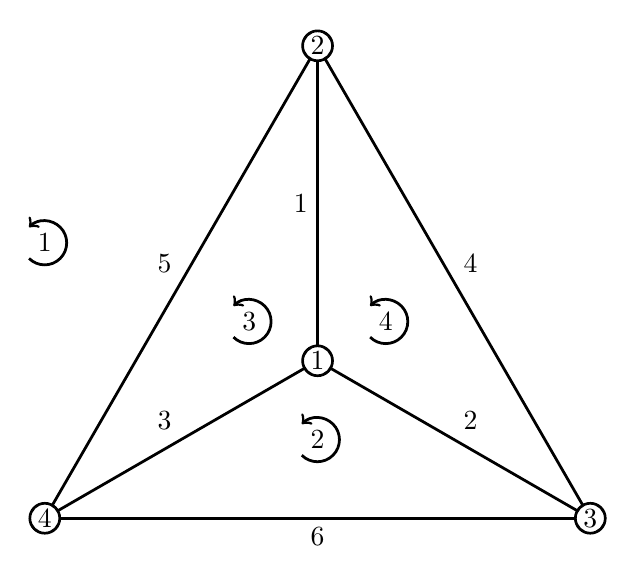
\begin{tikzpicture}[scale=4]

\coordinate (A) at (0,0);
\coordinate (B) at (0,1);
\coordinate (C) at (0.866,-0.5);
\coordinate (D) at (-0.866,-0.5);

\coordinate (b) at (0,-0.25);
\coordinate (c) at (-0.217,0.125);
\coordinate (d) at (0.217,0.125);
\coordinate (a) at (-0.866,0.375);

\coordinate (E) at (0,0.5);
\coordinate (F) at (0.433,-0.25);
\coordinate (G) at (-0.433,-0.25);
\coordinate (H) at (0.433,0.25);
\coordinate (I) at (-0.433,0.25);
\coordinate (J) at (0,-0.5);

\draw[line width=1pt] (A)--(B);
\draw[line width=1pt] (A)--(C);
\draw[line width=1pt] (A)--(D);
\draw[line width=1pt] (B)--(C);
\draw[line width=1pt] (B)--(D);
\draw[line width=1pt] (C)--(D);

\draw[fill=black] (A) circle[radius=0.5mm,fill]{};
\draw[fill=white] (A) circle[radius=0.45mm,fill]{};
\node at (A) {$1$};

\draw[fill=black] (B) circle[radius=0.5mm,fill]{};
\draw[fill=white] (B) circle[radius=0.45mm,fill]{};
\node at (B) {$2$};

\draw[fill=black] (C) circle[radius=0.5mm,fill]{};
\draw[fill=white] (C) circle[radius=0.45mm,fill]{};
\node at (C) {$3$};

\draw[fill=black] (D) circle[radius=0.5mm,fill]{};
\draw[fill=white] (D) circle[radius=0.45mm,fill]{};
\node at (D) {$4$};

\node at (b) {$2$};
\draw[->,line width=1pt] (b) + (-0.5mm,-0.5mm)
	arc[x radius=0.7mm,y radius=0.7mm,start angle=-135,end angle=135];
\node at (c) {$3$};
\draw[->,line width=1pt] (c) + (-0.5mm,-0.5mm)
	arc[x radius=0.7mm,y radius=0.7mm,start angle=-135,end angle=135];
\node at (d) {$4$};
\draw[->,line width=1pt] (d) + (-0.5mm,-0.5mm)
	arc[x radius=0.7mm,y radius=0.7mm,start angle=-135,end angle=135];
\node at (a) {$1$};
\draw[->,line width=1pt] (a) + (-0.5mm,-0.5mm)
	arc[x radius=0.7mm,y radius=0.7mm,start angle=-135,end angle=135];

\node at (E) [left] {$1$};
\node at (F) [above right] {$2$};
\node at (G) [above left] {$3$};
\node at (H) [above right] {$4$};
\node at (I) [above left] {$5$};
\node at (J) [below] {$6$};

\end{tikzpicture}
\caption{Netzwerk eines Tetraeders
\label{homologie:fig:tetragrid}}
\end{figure}

Wir berechnen die Homologie-Vektorräume für ein Tetraeder.
Ein Tetraeder besteht aus vier Dreiecken, die an den Kanten
verbunden sind.
In Abbildung~\ref{homologie:fig:tetragrid} ist das Tetraeder
schematisch dargestellt.
Die Seitenflächen sind numeriert mit den Zahlen, die von kreisförmligen
Pfeilen umgeben sind, die Seitenfläche $1$ soll man sich als die Bodenfläch
des Tetraeders vorstellen.
Die Kanten sind immer von der Ecke mit der kleineren Nummer zur
Ecke mit der grösseren Nummer orientiert.
Die Orientierung der Seitenflächen ist durch die kreisförmigen Pfeile
gegeben.

Aus dem Netzwerk~\ref{homologie:fig:tetragrid} können wir jetzt die
Randoperatoren ableiten.
Der Randoperator $\partial_1$ kann als $4\times 6$-Matrix dargestellt sind,
mit einer Zeile für jede Ecke und einer Spalte für jede Kante des
Tetraeders.
Anfangspunkte einer Kante werden mit $-1$ markiert, Endpunkte mit $1$.
So entsteht die Matrix
\[
\partial_1
=
\begin{pmatrix}
-1&-1&-1& 0& 0& 0\\
 1& 0& 0&-1&-1& 0\\
 0& 1& 0& 1& 0&-1\\
 0& 0& 1& 0& 1& 1
\end{pmatrix}.
\] 
Da die Summe jeder Spalten $0$ ist, kann $\partial_1$ nicht vollen Rang
haben.
Durch Nachrechnen findet man, dass $\operatorname{Rang}\partial_1=3$.

Der Randoperator $\partial_2$ berechnet aus jeder Seitenfläche die Summe
der orientierten Kanten, die die Seitenfläche beranden.
Wir können $\partial_2$ codieren als $6\times 4$-Matrix mit einer Zeile
für jede Kante und einer Spalte für jede Seitenfläche.
Die Kanten, die eine Seitenfläche beranden, werden mit $1$ markiert,
wenn ihre Orientierung mit der Pfeilrichtung der Seitenfläche übereinstimmt.
So erhalten wir die Matrix
\[
\partial_2
=
\begin{pmatrix}
 0& 0& 1&-1\\
 0&-1& 0& 1\\
 0& 1&-1& 0\\
 1& 0& 0&-1\\
-1& 0& 1& 0\\
 1&-1& 0& 0
\end{pmatrix}.
\]
Auch diese Matrix kann nicht vollen Rang haben, da jede Zeilensumme $0$ ist.
Tatsächlich zeigt die Rechnung dass $\operatorname{Rang}\partial_2 = 3$.

Durch Nachrechnen kann man auch kontrollieren, dass $\partial_1\partial_2=0$,
wie man das für einen Randoperator erwartet.
Daher ist $\operatorname{im}\partial_2\subset \operatorname{ker}\partial_1$.
Wir können jetzt die Dimensionen von Kern und Bild jedes Randoperators 
berechnen, und damit auch die Dimensionen der Homologie-Vektorräume.
\[
\begin{tikzcd}
	&\operatorname{dim}C_0=4
		&\operatorname{dim}C_1=6
			&\operatorname{dim}C_2=4
				&\operatorname{dim}C_3=0
\\
0
	&C_0 \ar[l,"\partial_0"]
		&C_1 \ar[l,"\partial_1"]
			&C_2 \ar[l,"\partial_2"]
				&0 \ar[l,"\partial_3"]
\\
	&{\textstyle \dim\operatorname{ker}\partial_0 = 4\atop
	 \textstyle \dim\operatorname{im}\partial_1 = 3}
		&{\textstyle\dim\operatorname{ker}\partial_1 = 3\atop
		  \textstyle\dim\operatorname{im}\partial_2 = 3}
			&{\textstyle\dim\operatorname{ker}\partial_2 = 1\atop
			  \textstyle\dim\operatorname{im}\partial_3 = 0}
\\
	&b_0=\dim H_0=1
		&b_1=\dim H_1=0
			&b_2=\dim H_2=1
\end{tikzcd}
\]
Die Bettizahlen $b_i$ führen uns auf die Euler-Charaketeristik
\[
\chi(\text{Tetraeder})
=
1 - 0 + 1 = 2,
\]
wie wir auch von der Rechnung mit dem Eulerschen Polyedersatz
aus der Einleitung dieses Abschnitts wissen.



%
% projektiv.tex
%
% (c) 2017 Prof Dr Andreas Müller, Hochschule Rapperswil
%
\subsection{Kleinsche Flasche}
Eine Kleinsche Flasche ist eine Fläche, die sich selbst durchdringt.
Die Fläche hat nur ein Seite und keinen Rand.
Wir können die Fläche mit einem Netzwerk von Dreiecken überziehen
und die Homologievektorräume berechnen oder mindestens deren Dimensionen
berechnen.
Dies ist jedoch einfacher, wenn man die Kleinsche Flasche aus einfacheren
Flächen zusammensetzen, die entsprechend einfachere Dreiecksnetze
haben.

Ein Möbius-Band entsteht, wenn man eine Streifen Papier eine halbe 
Drehung verdreht zusammenklebt.
Das Möbiusband hat nur eine Seite und nur eine Kante.
Man kann also ein Möbius-Band entlang dieses Randes mit einer
Kreisscheibe zusammenkleben.
Es stellt sich heraus, dass dadurch eine Kleinsche Flasche entsteht.
Der Plan ist also, eine Triangulation von Kreisscheibe und Möbiusband
zu finden, die am Rande zusammenpassen.
Daraus können wir dann die Randoperatoren und letztlich die Betti-Zahlen
berechnen.

\begin{figure}
\centering
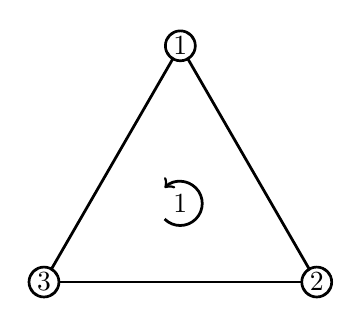
\begin{tikzpicture}[scale=4]
\coordinate (A) at (0,0.5);
\coordinate (B) at (0.433,-0.25);
\coordinate (C) at (-0.433,-0.25);
\draw[line width=1pt] (A)--(B);
\draw[line width=1pt] (A)--(C);
\draw[line width=1pt] (B)--(C);
\draw[fill=black] (A) circle[radius=0.5mm,fill]{};
\draw[fill=white] (A) circle[radius=0.45mm,fill]{};
\node at (A) {$1$};
\draw[fill=black] (B) circle[radius=0.5mm,fill]{};
\draw[fill=white] (B) circle[radius=0.45mm,fill]{};
\node at (B) {$2$};
\draw[fill=black] (C) circle[radius=0.5mm,fill]{};
\draw[fill=white] (C) circle[radius=0.45mm,fill]{};
\node at (C) {$3$};
\node at (0,0) {$1$};
\draw[->,line width=1pt] (-0.5mm,-0.5mm)
	arc[x radius=0.7mm,y radius=0.7mm,start angle=-135,end angle=135];
\end{tikzpicture}
\caption{Triangulation der Kreisscheibe
\label{homologie:fig:disk}}
\end{figure}

\begin{figure}
\centering
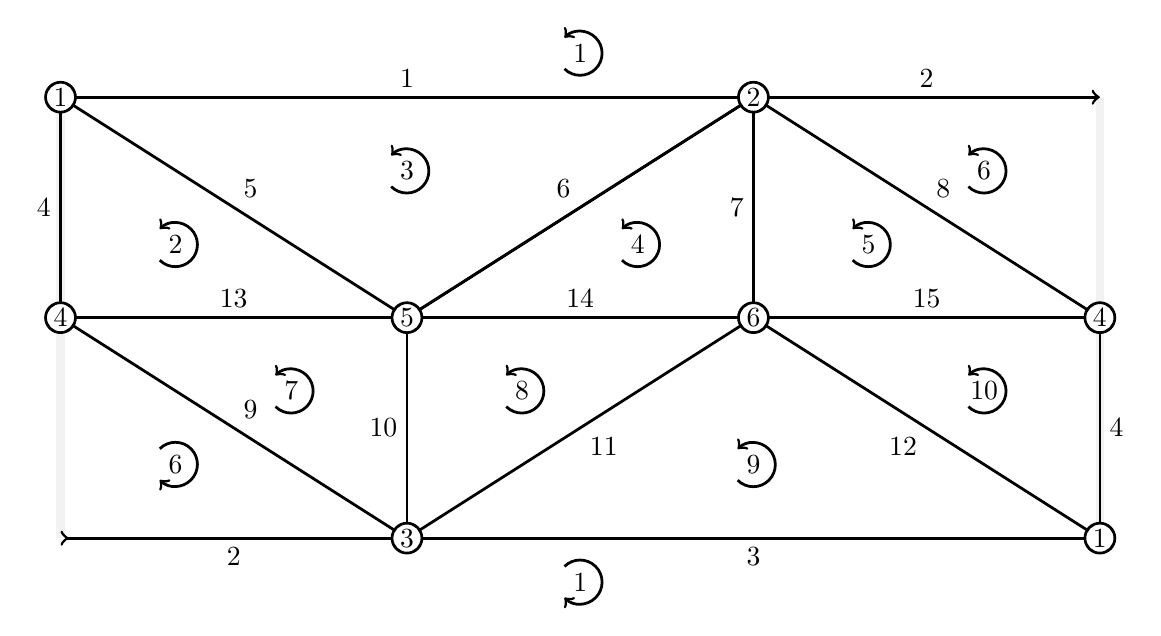
\begin{tikzpicture}[scale=4]
\def\w{2.2}
\def\h{1.4}
\coordinate (A) at ({0 * \w},{0.5 * \h});
\coordinate (a) at ({1.5 * \w},{-0.5 * \h});
\coordinate (B) at ({1 * \w},{0.5 * \h});
\coordinate (C) at ({0.5 * \w},{-0.5 * \h});
\coordinate (D) at ({0 * \w},{0 * \h});
\coordinate (E) at ({0.5 * \w},{0 * \h});
\coordinate (F) at ({1 * \w},{0 * \h});
\coordinate (d) at ({1.5 * \w},{0 * \h});
\draw[line width=3pt,color=gray!10] (A)--({0 * \w},{-0.5 * \h});
\draw[line width=3pt,color=gray!10] (a)--({1.5 * \w},{0.5 * \h});

\draw[->,line width=1pt] (A)--({1.5 * \w},{0.5 * \h});
\draw[>-,line width=1pt] ({0 * \w},{-0.5 * \h})--(a);

\draw[line width=1pt] (A)--(D);
\draw[line width=1pt] (A)--(E);
\draw[line width=1pt] (D)--(E);

\draw[line width=1pt] (B)--(E);
\draw[line width=1pt] (B)--(F);
\draw[line width=1pt] (E)--(F);

\draw[line width=1pt] (B)--(E);
\draw[line width=1pt] (B)--(d);
\draw[line width=1pt] (E)--(d);

\draw[line width=1pt] (D)--(C);
\draw[line width=1pt] (E)--(C);

\draw[line width=1pt] (C)--(F);
\draw[line width=1pt] (F)--(a);

\draw[line width=1pt] (a)--(d);

\draw[fill=black] (A) circle[radius=0.5mm,fill]{};
\draw[fill=white] (A) circle[radius=0.45mm,fill]{};
\node at (A) {$1$};

\draw[fill=black] (B) circle[radius=0.5mm,fill]{};
\draw[fill=white] (B) circle[radius=0.45mm,fill]{};
\node at (B) {$2$};

\draw[fill=black] (C) circle[radius=0.5mm,fill]{};
\draw[fill=white] (C) circle[radius=0.45mm,fill]{};
\node at (C) {$3$};

\draw[fill=black] (a) circle[radius=0.5mm,fill]{};
\draw[fill=white] (a) circle[radius=0.45mm,fill]{};
\node at (a) {$1$};

\draw[fill=black] (D) circle[radius=0.5mm,fill]{};
\draw[fill=white] (D) circle[radius=0.45mm,fill]{};
\node at (D) {$4$};

\draw[fill=black] (E) circle[radius=0.5mm,fill]{};
\draw[fill=white] (E) circle[radius=0.45mm,fill]{};
\node at (E) {$5$};

\draw[fill=black] (F) circle[radius=0.5mm,fill]{};
\draw[fill=white] (F) circle[radius=0.45mm,fill]{};
\node at (F) {$6$};

\draw[fill=black] (d) circle[radius=0.5mm,fill]{};
\draw[fill=white] (d) circle[radius=0.45mm,fill]{};
\node at (d) {$4$};

\def\flaeche#1#2{%
\node at #1 {#2};
\draw[->,line width=1pt] #1 + (-0.5mm,-0.5mm)
	arc[x radius=0.7mm,y radius=0.7mm,start angle=-135,end angle=135];
}

\def\rflaeche#1#2{%
\node at #1 {#2};
\draw[->,line width=1pt] #1 + (-0.5mm,0.5mm)
	arc[x radius=0.7mm,y radius=0.7mm,start angle=135,end angle=-135];
}

\flaeche{({0.166*\w},{0.166*\h})}{$2$};
\flaeche{({0.5*\w},{0.333*\h})}{$3$};
\flaeche{({0.833*\w},{0.166*\h})}{$4$};
\flaeche{({1.166*\w},{0.166*\h})}{$5$};
\flaeche{({1.333*\w},{0.333*\h})}{$6$};
\flaeche{({0.333*\w},{-0.166*\h})}{$7$};
\flaeche{({0.666*\w},{-0.166*\h})}{$8$};
\flaeche{({1*\w},{-0.333*\h})}{$9$};
\flaeche{({1.333*\w},{-0.166*\h})}{$10$};

\rflaeche{({0.166*\w},{-0.333*\h})}{$6$};
%\node at ({0.166*\w},{-0.333*\h}) {$6$};
%\draw[->,line width=1pt]
%	({0.166*\w},{-0.333*\h}) +(-0.5mm,0.5mm)
%	arc[x radius=0.7mm,y radius=0.7mm,start angle=135,end angle=-135];

\flaeche{({0.75*\w},{0.6*\h})}{$1$};
\rflaeche{({0.75*\w},{-0.6*\h})}{$1$};

\node at ({0.5*\w},{0.5*\h}) [above] {$1$};
\node at ({1.25*\w},{0.5*\h}) [above] {$2$};
\node at ({1*\w},{-0.5*\h}) [below] {$3$};
\node at ({0.25*\w},{-0.5*\h}) [below] {$2$};

\node at ({0*\w},{0.25*\h}) [left] {$4$};
\node at ({0.25*\w},{0.25*\h}) [above right] {$5$};
\node at ({0.75*\w},{0.25*\h}) [above left] {$6$};
\node at ({1*\w},{0.25*\h}) [left] {$7$};
\node at ({1.25*\w},{0.25*\h}) [above right] {$8$};

\node at ({0.25*\w},{-0.25*\h}) [above right] {$9$};
\node at ({0.5*\w},{-0.25*\h}) [left] {$10$};
\node at ({0.75*\w},{-0.25*\h}) [below right] {$11$};
\node at ({1.25*\w},{-0.25*\h}) [below left] {$12$};
\node at ({1.5*\w},{-0.25*\h}) [right] {$4$};

\node at ({0.25*\w},0) [above] {$13$};
\node at ({0.75*\w},0) [above] {$14$};
\node at ({1.25*\w},0) [above] {$15$};

\end{tikzpicture}
\caption{Triangulation des Möbisubandes
\label{homologie:fig:moebius}}
\end{figure}

\subsubsection{Triangulation der Kleinschen Flasche}
Die Kreisscheibe können wir als einfaches Dreieck triangulieren, wie
es in Abbildung~\ref{homologie:fig:klein} dargestellt ist.
Wie in früheren Beispielen sind die Kanten von kleineren Eckennummern
zu grösseren Eckennummern orientiert.
Das Möbiusband ist etwas komplizierter zu triangulieren.
Eine Möglichkeit ist in Abbildung~\ref{homologie:fig:klein} dargestellt.


\subsubsection{Randoperatoren}
Die Randoperatoren für die Kleinsche Flasche können jetzt aus
den Abbildungen \ref{homologie:fig:disk} und \ref{homologie:fig:moebius}
abgelesen werden.
Den $15$ Kanten werden jeweils zwei der $6$ Ecken zugeordnet, wie
durch die Matrix
\[
\setcounter{MaxMatrixCols}{15}
\partial_1
=
\begin{pmatrix}
%1  2  3  4  5  6  7  8  9 10 11 12 13 14 15
-1& 0&-1&-1&-1& 0& 0& 0& 0& 0& 0&-1& 0& 0& 0\\
 1&-1& 0& 0& 0&-1&-1&-1& 0& 0& 0& 0& 0& 0& 0\\
 0& 1& 1& 0& 0& 0& 0& 0&-1&-1&-1& 0& 0& 0& 0\\
 0& 0& 0& 1& 0& 0& 0& 1& 1& 0& 0& 0&-1& 0&-1\\
 0& 0& 0& 0& 1& 1& 0& 0& 0& 1& 0& 0& 1&-1& 0\\
 0& 0& 0& 0& 0& 0& 1& 0& 0& 0& 1& 1& 0& 1& 1
\end{pmatrix}
\]
beschrieben.
Der Randoperator $\partial_2$ ordnet jeder der Seitenfläche eine Summe
von Kanten zu mit positivem Vorzeichen jeweils dann, wenn die Kante gleich
orientiert ist wie der Pfeil der Seitenfläche anzeigt.
Die so definiert $15\times 10$-Matrix ist
\[
\partial_2
=
\begin{pmatrix}
%1  2  3  4  5  6  7  8  9 10
 1& 0&-1& 0& 0& 0& 0& 0& 0& 0	\\ %  1
 1& 0& 0& 0& 0&-1& 0& 0& 0& 0	\\ %  2
-1& 0& 0& 0& 0& 0& 0& 0&-1& 0	\\ %  3
 0& 1& 0& 0& 0& 0& 0& 0& 0& 1	\\ %  4
 0&-1& 1& 0& 0& 0& 0& 0& 0& 0	\\ %  5
 0& 0&-1& 1& 0& 0& 0& 0& 0& 0	\\ %  6
 0& 0& 0&-1& 1& 0& 0& 0& 0& 0	\\ %  7
 0& 0& 0& 0&-1& 1& 0& 0& 0& 0	\\ %  8
 0& 0& 0& 0& 0&-1&-1& 0& 0& 0	\\ %  9
 0& 0& 0& 0& 0& 0& 1&-1& 0& 0	\\ % 10
 0& 0& 0& 0& 0& 0& 0& 1&-1& 0	\\ % 11
 0& 0& 0& 0& 0& 0& 0& 0& 1&-1	\\ % 12
 0& 1& 0& 0& 0& 0&-1& 0& 0& 0	\\ % 13
 0& 0& 0& 1& 0& 0& 0&-1& 0& 0	\\ % 14
 0& 0& 0& 0&-1& 0& 0& 0& 0& 1	\\ % 15
\end{pmatrix}
\]
Beide Operatoren haben nicht vollen Rang, die Berechnung ergibt
\[
\operatorname{Rang}\partial_1 = 5
\qquad\text{und}\qquad
\operatorname{Rang}\partial_2 = 10.
\]
Durch Nachrechnen überprüft man auch $\partial_1\partial_2=0$, also
$\operatorname{im}\partial_2\subset \operatorname{ker}\partial_1$.

\subsubsection{Homologie einer Kleinschen Flasche}
Aus den bekannten Randoperatoren $\partial_1$ und $\partial_2$ kann
man jetzt die Dimensionen der Homologievektorräume berechnen:
\[
\begin{tikzcd}
	&\operatorname{dim}C_0 = 6
		&\operatorname{dim}C_1 = 15
			&\operatorname{dim}C_2 = 10
				&
\\
0
	&C_0 \ar[l,"\partial_0"]
		&C_1 \ar[l,"\partial_1"]
			&C_2 \ar[l,"\partial_2"]
				&0
\\
	&{\textstyle\dim\operatorname{ker}\partial_0=6\atop
	  \textstyle\dim\operatorname{im}\partial_1=5}
		&{\textstyle\dim\operatorname{ker}\partial_1=10\atop
		  \textstyle\dim\operatorname{im}\partial_2=10}
			&{\textstyle\dim\operatorname{ker}\partial_2=0\atop
			  \textstyle\dim\operatorname{im}\partial_3=0}
\\
	&\dim H_0 = 1
		&\dim H_1 = 0
			&\dim H_2 = 0
\end{tikzcd}
\]
Aus sicht der reellen Homologie-Vektorräume ist die Kleinsche Flasche
also nicht von einem Punkt unterscheidbar.
Betrachtet man allerdings alle Vektorräume als Vektorräume über
$\mathbb F_2$, dann ergibt sich ein anderes Bild.
In den Matrizen $\partial_1$ und $\partial_2$ ist dann $-1$ durch $1$
zu ersetzen.
Die Berechnung des Ranges ergibt
\[
\operatorname{Rang}\partial_1 = 5
\qquad\text{und}\qquad
\operatorname{Rang}\partial_2 = 9
\]
Die Dimensionen der Homologie-Vektorräume sind
\[
\begin{tikzcd}
	&\operatorname{dim}C_0 = 6
		&\operatorname{dim}C_1 = 15
			&\operatorname{dim}C_2 = 10
				&
\\
0
	&C_0 \ar[l,"\partial_0"]
		&C_1 \ar[l,"\partial_1"]
			&C_2 \ar[l,"\partial_2"]
				&0
\\
	&{\textstyle\dim\operatorname{ker}\partial_0=6\atop
	  \textstyle\dim\operatorname{im}\partial_1=5}
		&{\textstyle\dim\operatorname{ker}\partial_1=10\atop
		  \textstyle\dim\operatorname{im}\partial_2=9}
			&{\textstyle\dim\operatorname{ker}\partial_2=1\atop
			  \textstyle\dim\operatorname{im}\partial_3=0}
\\
	&\dim H_0 = 1
		&\dim H_1 = 1
			&\dim H_2 = 1
\end{tikzcd}
\]
Der Unterschied stammt daher, dass die $\mathbb F_2$-Homologie zwischen
$1$ und $-1$ nicht unterschieden kann, also die Orientierung der
Flächen und Kanten ignoriert.
Die $\mathbb R$-Homologie dagegen kann die beiden Orientierungen
unterschieden.







%
% algtopo.tex -- Intro in die algebraische Topologie
%
% (c) 2017 Prof Dr Andreas Müller, Hochschule Rapperswil
%
\section{Algebraische Topologie}
Die in diesem Kapitel gezeigte elementare Homologietheorie ist ein
erster Schritt in das weite Gebiet der algebraischen Topologie.
Diese befasst sich mit den Eigenschaften geometrischer Objekte, die
sich unter Deformationen nicht ändern.
Das Grundprinzip ist, einem geometrischen Objekt ein algebraisches Objekt
zuzuordnen.
Zum Beispiel haben wir gesehen, wie man einem Polyeder oder allgemeiner
einem simplizialen Komplex $X$ eine Reihe von Vektorräumen $H_0(X,\mathbb R)$,
$H_1(X,\mathbb R),\dots$ zuordnet.
An verschiedenen Dimensionen dieser Vektorräume können wir bereits 
Unterschiede erkennen.

Die Dimension des Homologie-Vektorraumes $H_0(X,\mathbb R)$ gibt die Anzahl
der Zusammenhangskomponenten an.
Die Dimension von $H_1(X,\mathbb R)$ zählt die Zyklen, die 







